%\documentclass{cmspaper}
%\begin{document}

\section{Event Selection} \label{sec:eventSelection}

% Analysis strategy (M dist, bump search)
% Optimize signal, minimize bkgd
% Plots of selection variables
% (optimization of selection criteria)
% List of selection criteria (Mee, St, etc.)

The basic strategy to identify the existence of a particle that decays to a jet and an electron 
is to study the invariant mass of the electron-jet pairs in the events. 
The signal of a leptoquark would appear as a bump in the distribution of this invariant mass.
The decay of a particle to a jet and a lepton is forbidden in the standard model.  
Thus, a peak at the mass of the leptoquark would be the only resonance in this distribution. 
The electron-jet combinations of the background events have a different shape than that 
of the leptoquark resonance. 
Nonetheless, the number of background events could dominate over the number of signal events.  
The cut-based selection described in this section has been made in order to minimize the number 
of background events selected while retaining a high signal efficiency.

The decay of a leptoquark and an anti-leptoquark produces two high energy electrons and 
two high energy jets.
The online selection of candidate events is made by either the HLT trigger ``HLT\_Photon15\_L1R'' 
or ``HLT\_Photon25\_L1R'' described in section~\ref{sec:trig}, depending on the luminosity scenario, 
while the offline identification of electrons and jets 
proceeds as described in sections~\ref{sec:electrons} and \ref{sec:jet}, respectively.

%FIXME add skim
In order to reduce the size of the of the data samples and the time to analyze them, a skim of the 
data has been defined.
The requirements that the skim has to satisfy have been defined considering that this skim may be needed
for the analysis of both first and second generation leptoquark pair production. Such requirements are:
\begin{itemize}
\item having a high efficiency for first (events with 2 electrons and 2 jets) and second (events with 
2 muons and 2 jets) generation leptoquark pair production; 
\item keeping events needed for the control samples: the control sample for the Z+jets background is $Z\rightarrow l l$+ 2 jets,
where $l$ is is either an electron or a muon; the control sample for the the $t\bar{t}$+jets background is a sample 
with an electron, a muon and 2 jets;
\item suppressing all other backgrounds
\end{itemize}
The cuts that define the skim have been chosen as:
\begin{itemize}
\item $N_l \equiv N_e + N_{\mu} \ge 2$, where $N_e (N_{\mu})$ is the number of reconstructed electrons (muons)
with $P_T>20~$GeV and without ID or isolation requirements applied; this cut suppresses events with low 
lepton multiplicity and low lepton $P_T$, such as QCD, W+jets and $t\bar{t}$ fully hadronic decays;
\item $N_{\mathrm{obj}} \ge 4$, where $N_{\mathrm{obj}} \equiv N_l + N_{\mathrm{jet}}$; $N_l$ is defined as above, and
$N_{\mathrm{jet}}$ is the number of the jets with a raw (i.e. without jet energy corrections) $P_T > 10~$GeV and without 
any electron with $P_T > 20~$GeV within a cone of $\Delta R=0.1$; this cut suppresses $Z \rightarrow ll$ and 
$Z \rightarrow ll$+~1~jet while preserving $Z \rightarrow ll$+~2~(or more)~jets.
\end{itemize}

Number of events in the skimmed sample with 100 $pb^{-1}$ of data, and 
efficiency of the skim for signal and background are shown in the second line (``Skim'') 
of Tables
\ref{tab:effic-MLQ400}, 
\ref{tab:effic-ttbar}, 
\ref{tab:effic-Z}, 
\ref{tab:effic-QCD},
\ref{tab:effic-VV} and
\ref{tab:effic-W}.

The offline selection of the eejj sample continues with the following kinematic cuts:
%
\begin{enumerate}
\item at least 2 isolated electrons, both of them required $P_T>30$~GeV 
\item at least 2 jets, both of them required to have $P_T>50$~GeV and $|\eta|<3$
\item $M_{ee}>100$~GeV
\item $S_T\equiv P_T(e_1)+P_T(e_2)+P_T(j_1)+P_T(j_2)>f(M_{LQ})$, where $f(M_{LQ})$ is a function 
of the hypothesized LQ mass.
\end{enumerate}
%

The specific values of the kinematic cuts has been determined using a cut-optimization procedure meant to
reach the maximum potential of the analysis for excluding the existence of a LQ signal. 
Such a procedure is described in section~\ref{sec:cutOptimization}.

Cut 1 and 2 set a minimum value on the transverse momentum of electrons and jets. 
The 2 leading electrons and 2 leading jets are used to continue the selection.
Cut 3, where $M_{ee}$ is the invariant mass of the electron pair, removes background events from 
$Z/\gamma$+jets events as shown in figure~\ref{fig:Mee_St_distributions}-left.
Cut 4, where the variable $S_T$ is defined as the scalar sum of the transverse momenta of the 
2 electrons and 2 jets, is applied following the approach of the experiment $D0$ in 
\cite{Abazov:2001mx}. In that paper, an event selection optimization as a function of
the combinations of several kinematic variables has shown that $S_T$ is the most powerful one 
and little is gained by adding cuts on other variables. The distribution of $S_T$ for the present
analysis is shown in figure~\ref{fig:Mee_St_distributions}-right.

Once the eejj sample is selected, there are two ways to combine two electrons and two jets to make two electron-jet pairs. 
For each event, the combination with the minimum difference, $\Delta M_{ej}$, between the invariant masses, $M_{ej}$, 
of the two electron-jet pairs is chosen\footnote{
A study at MC generator level has been performed to investigate the effect of jets generated by initial state 
radiation (ISR). The probability that an ISR jet has actually a larger $P_T$ than one or both jets produced 
by the decay of the leptoquarks is 25\% and 12\% at LQ mass of 250~GeV, and 20\% and 8\% at LQ mass of 400~GeV. 
In such percentage of events, choosing the 2 leading jets as daughters of the leptoquarks is not correct. 
If the third leading jet were considered, the number of combinations to make 2 electron-jet pairs would become six.
The same algorithm used above and based on the minimum difference $\Delta M_{ej}$ could be applied to select one 
among the six combinations. Our study showed that the improvement in finding the correct combination would be at the level
of the percent with respect to the case where only the two leading jets are considered.
%Using $\Delta M_{ej}$ divided by the average of the two $M_{ej}$ as discriminator quantity instead of $\Delta M_{ej}$
%would bring a further, but even minor improvement.
Given the moderate improvement coming from using the third leading jet and considerations of simplicity and robustness
of the analysis, the current version of the analysis uses only the two leading jets.
}. 
The resulting $M_{ej}$ distribution after the full selection is shown in figure~\ref{fig:Mej_allComb} for the signal and backgrounds. 

\begin{figure}[htbp]
  \begin{center}
    \begin{tabular}{cc}
      \resizebox{7.5cm}{!}{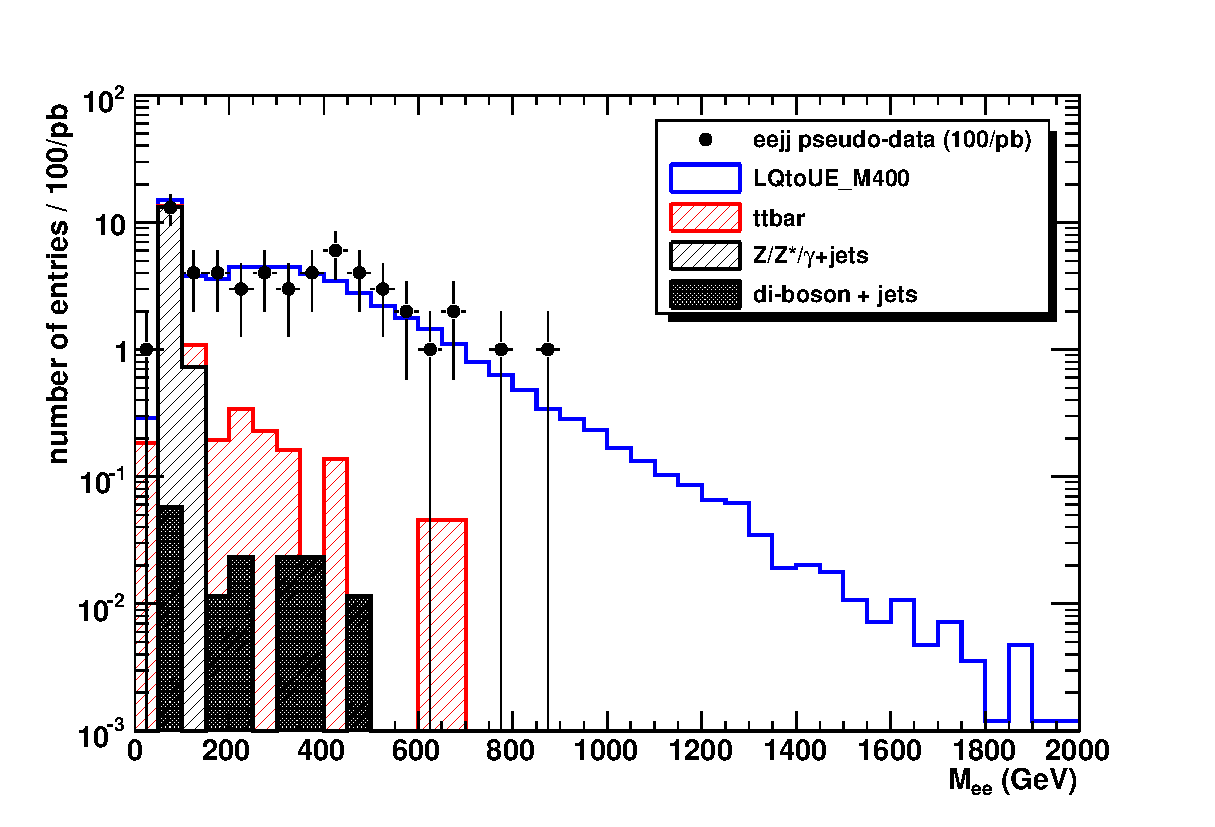
\includegraphics{plots/LQ400FullSimeejjFinalPlots/Mee_eejj_LQ400_100pb.eps}} &
      \resizebox{7.5cm}{!}{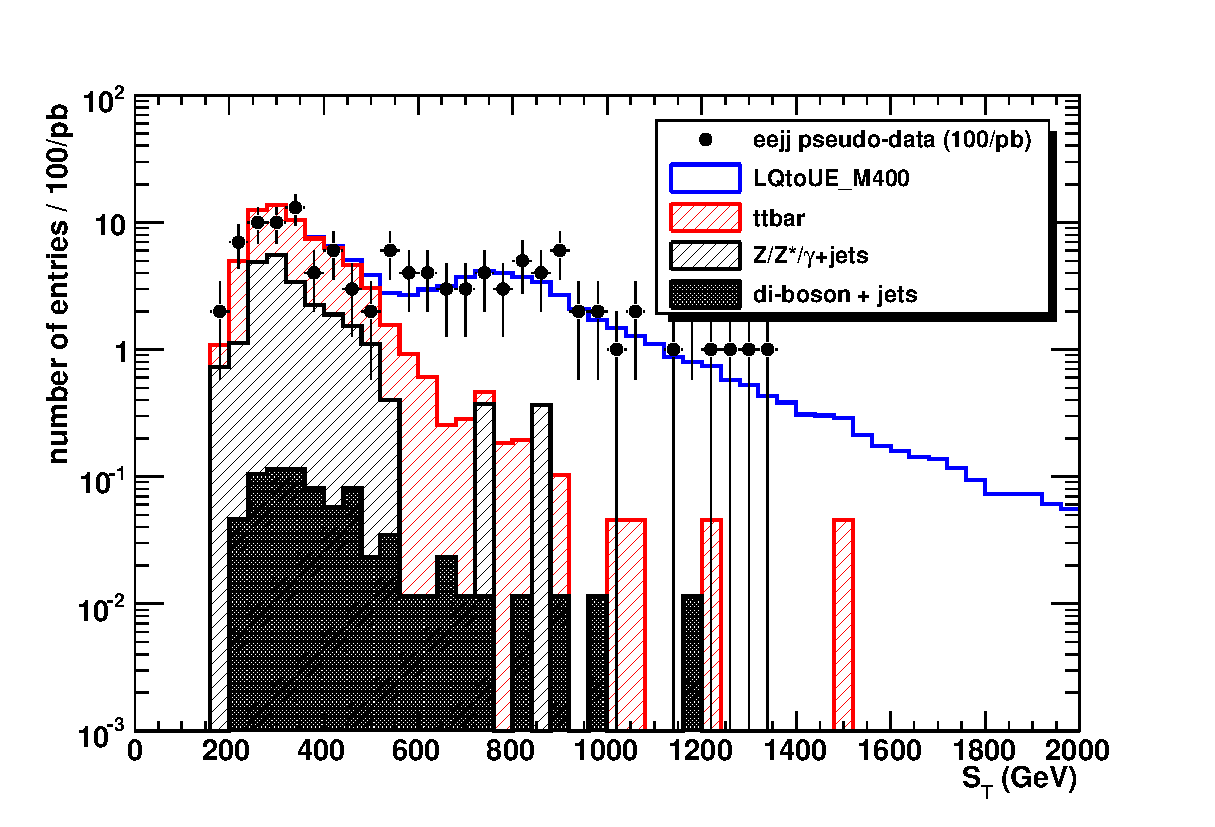
\includegraphics{plots/LQ400FullSimeejjFinalPlots/ST_eejj_LQ400_100pb.eps}} \\
    \end{tabular}
    \caption{\small \sl Left: invariant mass of the electron pair, $M_{ee}$. 
             Right: scalar sum of the $P_T$ of the 2 leading electrons and 2 leading jets. 
	     In each histogram, the distributions for the signal with $M_{LQ}=400~$GeV 
	     and the contributing backgrounds 
	     (with the exception of the QCD background, see Section~\ref{sec:QCDBackground}) are shown after 
	     applying all cuts except the one involving the plotted variable. 
	     All histograms are summed on top of each other.
	     }
    \label{fig:Mee_St_distributions}
  \end{center}
\end{figure}


\begin{figure}[htbp]
  \begin{center}
    \begin{tabular}{cc}
      \resizebox{7.5cm}{!}{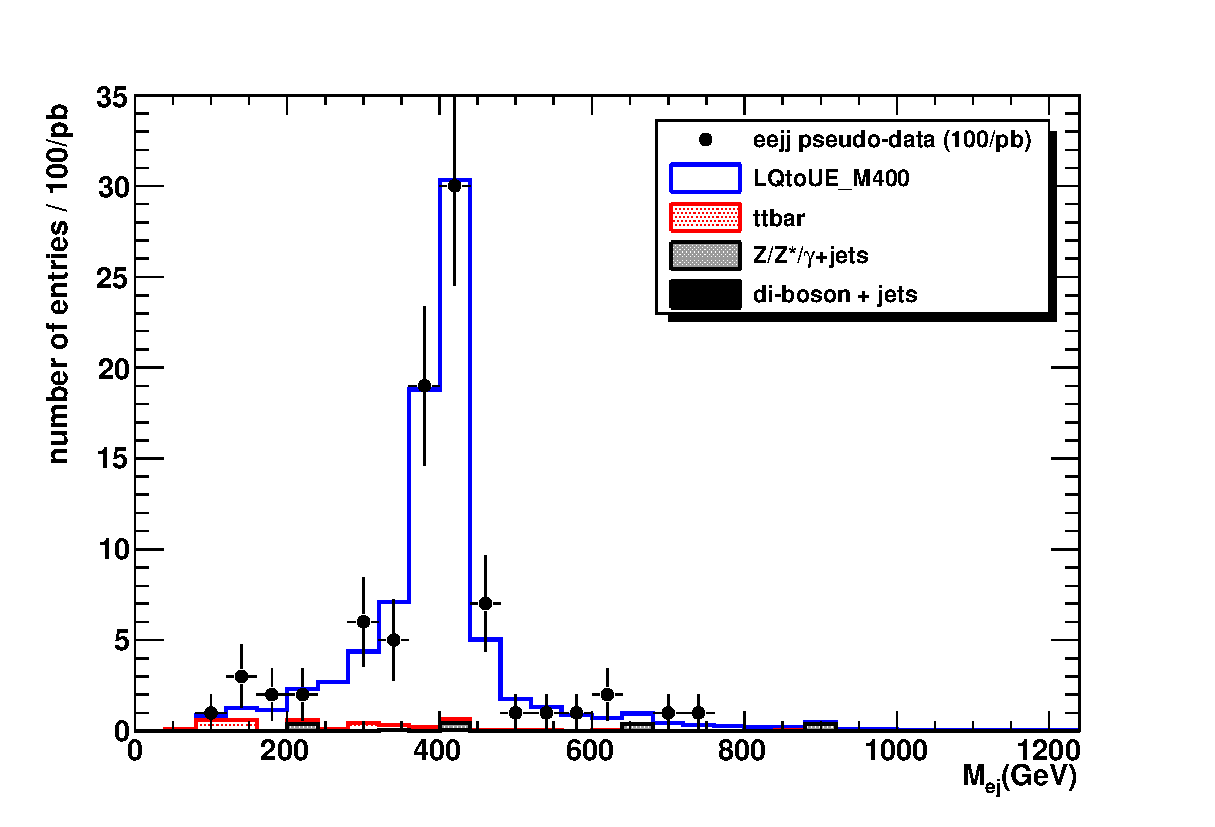
\includegraphics{plots/LQ400FullSimeejjFinalPlots/Mej_eejj_LQ400_100pb_LinScale.eps}} & 
      \resizebox{7.5cm}{!}{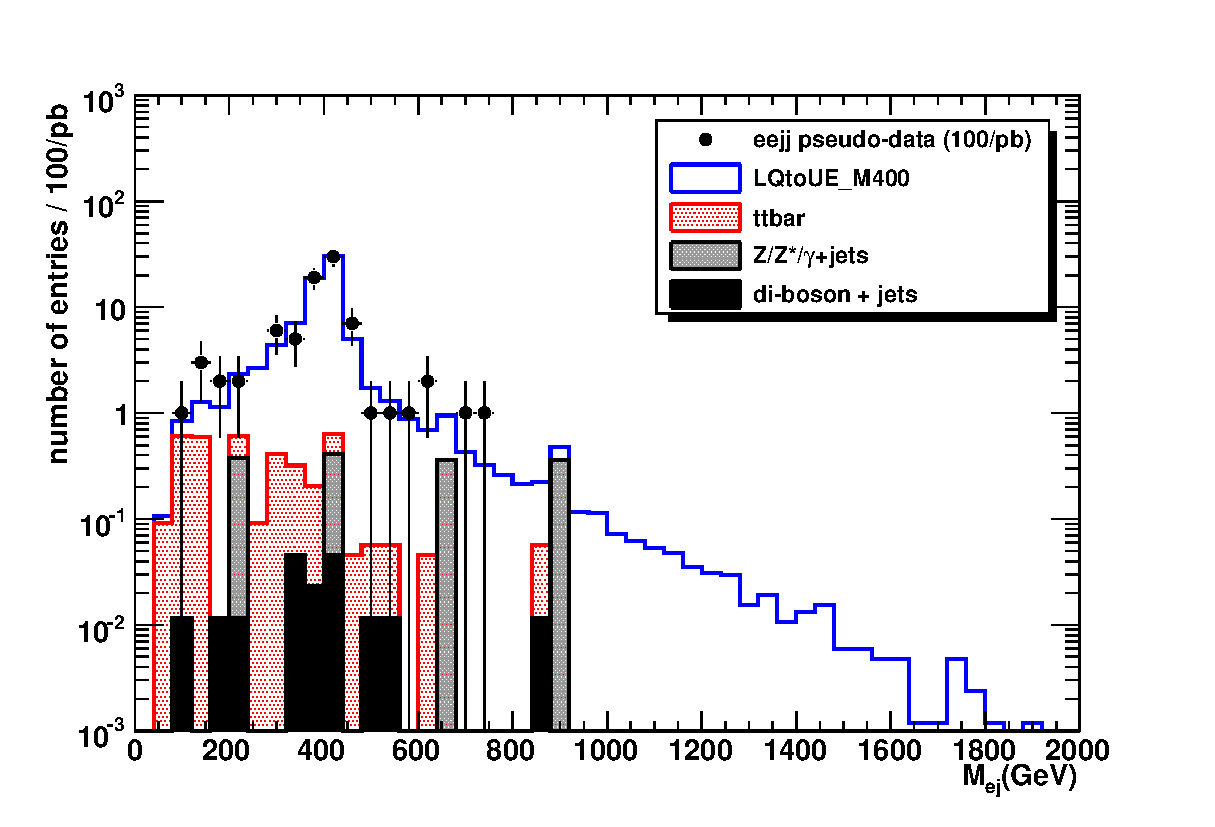
\includegraphics{plots/LQ400FullSimeejjFinalPlots/Mej_eejj_LQ400_100pb.eps}} \\
    \end{tabular}
    \caption{\small \sl Distribution of the invariant mass, $M_{ej}$, 
      of the electron-jet pairs with smaller $\Delta M_{ej}$ for the signal with $M_{LQ}=400~$GeV and the contributing backgrounds 
      (with the exception of the QCD background, see Section~\ref{sec:QCDBackground}). 
      The complete event selection has been applied.
      All histograms are summed on top of each other. 
      The plot is shown in linear and log scale on the left- and right-hand-side, respectively. 
      }
    \label{fig:Mej_allComb}
  \end{center}
\end{figure}



Tables  
\ref{tab:effic-MLQ400}, 
\ref{tab:effic-ttbar}, 
\ref{tab:effic-Z}, 
\ref{tab:effic-QCD},
\ref{tab:effic-VV} and
\ref{tab:effic-W}
show the efficiency of the selection cuts for signal events at $M_{LQ}=400~$GeV and the main background samples.
In all these tables, the $S_T$ cut is set to the value (620~GeV) optimized for this LQ mass.  

\begin{table}[htbp] 
\begin{center} 
\begin{tabular}{|c|c|c|c|} 
\hline\hline 
 Cut & $N_{evt}$ passed for $100pb^{-1}$ & $\varepsilon_{rel}$ & $\varepsilon_{abs}$ \\ 
\hline\hline 
None       &        7.50e+01       $~\pm~$       0.00e+00        &        1.0e+00       $~\pm~$       0.0e+00        &        1.0e+00       $~\pm~$       0.0e+00       \\       
       Skim       &        6.80e+01       $~\pm~$       9.00e-02        &        9.1e-01       $~\pm~$       1.3e-03        &        9.1e-01       $~\pm~$       1.2e-03       \\       
       2 ele $P_T>30~$GeV       &        6.68e+01       $~\pm~$       9.00e-02        &        9.8e-01       $~\pm~$       1.9e-03        &        8.9e-01       $~\pm~$       1.2e-03       \\       
       2 ele (ID+Iso) $P_T>30~$GeV       &        5.01e+01       $~\pm~$       1.40e-01        &        7.5e-01       $~\pm~$       3.1e-03        &        6.7e-01       $~\pm~$       1.9e-03       \\       
       2 jets (Cleaned),$P_T>$50~GeV,$|\eta|<$3       &        4.69e+01       $~\pm~$       1.40e-01        &        9.4e-01       $~\pm~$       4.1e-03        &        6.3e-01       $~\pm~$       1.9e-03       \\       
       $M_{ee}>$100~GeV       &        4.49e+01       $~\pm~$       1.50e-01        &        9.6e-01       $~\pm~$       4.5e-03        &        6.0e-01       $~\pm~$       1.9e-03       \\       
       $S_T>$620~GeV       &        3.90e+01       $~\pm~$       1.50e-01        &        8.7e-01       $~\pm~$       5.1e-03        &        5.2e-01       $~\pm~$       2.0e-03       \\       
          \hline\hline 
\end{tabular} 
\end{center} 
\caption{Sample of $M_{LQ}=400~$GeV (FullSim): Sequence of selection cuts with number of events selected in 100$~pb^{-1}$, efficiency relative to the preceding cut and absolute efficiency. The reported uncertainties on the number of events and efficiencies are statistical, due to the number of analyzed MC events.} 
\label{tab:effic-MLQ400} 
\end{table} 

\begin{table}[htbp] 
\begin{center} 
\begin{tabular}{|c|c|c|c|} 
\hline\hline 
 Cut & $N_{evt}$ passed for $100pb^{-1}$ & $\varepsilon_{rel}$ & $\varepsilon_{abs}$ \\ 
\hline\hline 
None       &        4.14e+04       $~\pm~$       0.00e+00        &        1.0e+00       $~\pm~$       0.0e+00        &        1.0e+00       $~\pm~$       0.0e+00       \\       
       Skim       &        6.75e+03       $~\pm~$       1.61e+01        &        1.6e-01       $~\pm~$       2.4e-03        &        1.6e-01       $~\pm~$       3.9e-04       \\       
       2 ele $P_T>30~$GeV       &        1.75e+03       $~\pm~$       8.77e+00        &        2.6e-01       $~\pm~$       5.5e-03        &        4.2e-02       $~\pm~$       2.1e-04       \\       
       2 ele (ID+Iso) $P_T>30~$GeV       &        1.55e+02       $~\pm~$       2.66e+00        &        8.8e-02       $~\pm~$       1.8e-02        &        3.7e-03       $~\pm~$       6.4e-05       \\       
       2 jets (Cleaned),$P_T>$50~GeV,$|\eta|<$3       &        7.72e+01       $~\pm~$       1.88e+00        &        5.0e-01       $~\pm~$       3.0e-02        &        1.9e-03       $~\pm~$       4.5e-05       \\       
       $M_{ee}>$100~GeV       &        4.62e+01       $~\pm~$       1.45e+00        &        6.0e-01       $~\pm~$       4.0e-02        &        1.1e-03       $~\pm~$       3.5e-05       \\       
       $S_T>$620~GeV       &        1.46e+00       $~\pm~$       2.60e-01        &        3.2e-02       $~\pm~$       1.8e-01        &        3.5e-05       $~\pm~$       6.3e-06       \\       
          \hline\hline 
\end{tabular} 
\end{center} 
\caption{Sample of $t\bar{t}$ + N jets: Sequence of selection cuts with number of events selected in 100$~pb^{-1}$, efficiency relative to the preceding cut and absolute efficiency.  The reported uncertainties on the number of events and efficiencies are statistical, due to the number of analyzed MC events.} 
\label{tab:effic-ttbar} 
\end{table} 

\begin{table}[htbp] 
\begin{center} 
\begin{tabular}{|c|c|c|c|} 
\hline\hline 
 Cut & $N_{evt}$ passed for $100pb^{-1}$ & $\varepsilon_{rel}$ & $\varepsilon_{abs}$ \\ 
\hline\hline 
None       &        4.22e+05       $~\pm~$       0.00e+00        &        1.0e+00       $~\pm~$       0.0e+00        &        1.0e+00       $~\pm~$       0.0e+00       \\       
       Skim       &        9.01e+03       $~\pm~$       5.67e+01        &        2.1e-02       $~\pm~$       6.3e-03        &        2.1e-02       $~\pm~$       1.3e-04       \\       
       2 ele $P_T>30~$GeV       &        2.65e+03       $~\pm~$       3.10e+01        &        2.9e-01       $~\pm~$       1.3e-02        &        6.3e-03       $~\pm~$       7.3e-05       \\       
       2 ele (ID+Iso) $P_T>30~$GeV       &        2.02e+03       $~\pm~$       2.70e+01        &        7.6e-01       $~\pm~$       1.8e-02        &        4.8e-03       $~\pm~$       6.4e-05       \\       
       2 jets (Cleaned),$P_T>$50~GeV,$|\eta|<$3       &        3.28e+02       $~\pm~$       1.09e+01        &        1.6e-01       $~\pm~$       3.6e-02        &        7.8e-04       $~\pm~$       2.6e-05       \\       
       $M_{ee}>$100~GeV       &        2.29e+01       $~\pm~$       2.89e+00        &        7.0e-02       $~\pm~$       1.3e-01        &        5.4e-05       $~\pm~$       6.8e-06       \\       
       $S_T>$620~GeV       &        7.30e-01       $~\pm~$       5.20e-01        &        3.2e-02       $~\pm~$       7.2e-01        &        1.7e-06       $~\pm~$       1.2e-06       \\       
          \hline\hline 
\end{tabular} 
\end{center} 
\caption{Sample of $Z/\gamma$ + N jets: Sequence of selection cuts with number of events selected in 100$~pb^{-1}$, efficiency relative to the preceding cut and absolute efficiency.  The reported uncertainties on the number of events and efficiencies are statistical, due to the number of analyzed MC events.} 
\label{tab:effic-Z} 
\end{table} 

\begin{table}[htbp] 
\begin{center} 
\begin{tabular}{|c|c|c|c|} 
\hline\hline 
 Cut & $N_{evt}$ passed for $100pb^{-1}$ & $\varepsilon_{rel}$ & $\varepsilon_{abs}$ \\ 
\hline\hline 
None       &        1.18e+03       $~\pm~$       0.00e+00        &        1.0e+00       $~\pm~$       0.0e+00        &        1.0e+00       $~\pm~$       0.0e+00       \\       
       Skim       &        6.31e+01       $~\pm~$       8.30e-01        &        5.3e-02       $~\pm~$       1.3e-02        &        5.3e-02       $~\pm~$       7.1e-04       \\       
       2 ele $P_T>30~$GeV       &        1.52e+01       $~\pm~$       4.20e-01        &        2.4e-01       $~\pm~$       3.1e-02        &        1.3e-02       $~\pm~$       3.5e-04       \\       
       2 ele (ID+Iso) $P_T>30~$GeV       &        9.49e+00       $~\pm~$       3.30e-01        &        6.2e-01       $~\pm~$       4.4e-02        &        8.0e-03       $~\pm~$       2.8e-04       \\       
       2 jets (Cleaned),$P_T>$50~GeV,$|\eta|<$3       &        1.65e+00       $~\pm~$       1.40e-01        &        1.7e-01       $~\pm~$       9.2e-02        &        1.4e-03       $~\pm~$       1.2e-04       \\       
       $M_{ee}>$100~GeV       &        8.00e-01       $~\pm~$       1.00e-01        &        4.8e-01       $~\pm~$       1.5e-01        &        6.8e-04       $~\pm~$       8.1e-05       \\       
       $S_T>$620~GeV       &        9.00e-02       $~\pm~$       3.00e-02        &        1.1e-01       $~\pm~$       3.6e-01        &        7.9e-05       $~\pm~$       2.8e-05       \\       
          \hline\hline 
\end{tabular} 
\end{center} 
\caption{Sample of $VV$ + N jets: Sequence of selection cuts with number of events selected in 100$~pb^{-1}$, efficiency relative to the preceding cut and absolute efficiency.  The reported uncertainties on the number of events and efficiencies are statistical, due to the number of analyzed MC events.} 
\label{tab:effic-VV} 
\end{table} 

\begin{table}[htbp]
\begin{center}
\begin{tabular}{|c|c|c|c|}
\hline\hline
 Cut & $N_{evt}$ passed for $100pb^{-1}$ & $\varepsilon_{rel}$ & $\varepsilon_{abs}$ \\
\hline\hline
None       &        4.56e+06       $~\pm~$       0.00e+00        &        1.0e+00       $~\pm~$       0.0e+00        &        1.0e+00       $~\pm~$       0.0e+00       \\       
       Skim       &        4.70e+03       $~\pm~$       5.92e+01        &        1.0e-03       $~\pm~$       1.3e-02        &        1.0e-03       $~\pm~$       1.3e-05       \\       
       2 ele $P_T>30~$GeV       &        1.17e+03       $~\pm~$       2.95e+01        &        2.5e-01       $~\pm~$       2.8e-02        &        2.6e-04       $~\pm~$       6.5e-06       \\       
       2 ele (ID+Iso) $P_T>30~$GeV       &        8.21e+00       $~\pm~$       2.48e+00        &        7.0e-03       $~\pm~$       3.0e-01        &        1.8e-06       $~\pm~$       5.4e-07       \\       
       2 jets (Cleaned),$P_T>$50~GeV,$|\eta|<$3       &        1.49e+00       $~\pm~$       1.06e+00        &        1.8e-01       $~\pm~$       7.7e-01        &        3.3e-07       $~\pm~$       2.3e-07       \\       
       $M_{ee}>$100~GeV       &        0.00e+00       $~\pm~$       0.00e+00        &        0.0e+00       $~\pm~$       7.1e-01        &        0.0e+00       $~\pm~$       0.0e+00       \\       
       $S_T>$620~GeV       &        0.00e+00       $~\pm~$       0.00e+00        &        0.0e+00       $~\pm~$       0.0e+00        &        0.0e+00       $~\pm~$       0.0e+00       \\       
          \hline\hline
\end{tabular}
\end{center}
\caption{Sample of W + N jets: Sequence of selection cuts with number of events selected in 100$~pb^{-1}$, efficiency relative to the preceding cut and absolute efficiency.  The reported uncertainties on the number of events and efficiencies are statistical, due to the number of analyzed MC events.}
\label{tab:effic-W}
\end{table}

\begin{table}[htbp] 
\begin{center} 
\begin{tabular}{|c|c|c|c|} 
\hline\hline 
 Cut & $N_{evt}$ passed for $100pb^{-1}$ & $\varepsilon_{rel}$ & $\varepsilon_{abs}$ \\ 
\hline\hline 
None       &        1.50e+09       $~\pm~$       0.00e+00        &        1.0e+00       $~\pm~$       0.0e+00        &        1.0e+00       $~\pm~$       0.0e+00       \\       
       Skim       &        5.11e+05       $~\pm~$       7.47e+03        &        3.4e-04       $~\pm~$       1.5e-02        &        3.4e-04       $~\pm~$       5.0e-06       \\       
       2 ele $P_T>30~$GeV       &        4.73e+04       $~\pm~$       2.27e+03        &        9.3e-02       $~\pm~$       5.0e-02        &        3.2e-05       $~\pm~$       1.5e-06       \\       
       2 ele (ID+Iso) $P_T>30~$GeV       &        1.09e+02       $~\pm~$       1.09e+02        &        2.3e-03       $~\pm~$       1.0e+00        &        7.3e-08       $~\pm~$       7.3e-08       \\       
       2 jets (Cleaned),$P_T>$50~GeV,$|\eta|<$3       &        0.00e+00       $~\pm~$       0.00e+00        &        0.0e+00       $~\pm~$       1.0e+00        &        0.0e+00       $~\pm~$       0.0e+00       \\       
       $M_{ee}>$100~GeV       &        0.00e+00       $~\pm~$       0.00e+00        &        0.0e+00       $~\pm~$       0.0e+00        &        0.0e+00       $~\pm~$       0.0e+00       \\       
       $S_T>$620~GeV       &        0.00e+00       $~\pm~$       0.00e+00        &        0.0e+00       $~\pm~$       0.0e+00        &        0.0e+00       $~\pm~$       0.0e+00       \\       
       \hline\hline 
\end{tabular} 
\end{center} 
\caption{Sample of QCD ($H_T \in [100,250]~$GeV): Sequence of selection cuts with number of events selected in 100$~pb^{-1}$, efficiency relative to the preceding cut and absolute efficiency. The reported uncertainties on the number of events and efficiencies are statistical, due to the number of analyzed MC events.} 
\label{tab:effic-QCD-100-250} 
\end{table} 

\begin{table}[htbp] 
\begin{center} 
\begin{tabular}{|c|c|c|c|} 
\hline\hline 
 Cut & $N_{evt}$ passed for $100pb^{-1}$ & $\varepsilon_{rel}$ & $\varepsilon_{abs}$ \\ 
\hline\hline 
None       &        4.00e+07       $~\pm~$       0.00e+00        &        1.0e+00       $~\pm~$       0.0e+00        &        1.0e+00       $~\pm~$       0.0e+00       \\       
       Skim       &        6.61e+05       $~\pm~$       2.65e+03        &        1.7e-02       $~\pm~$       4.0e-03        &        1.7e-02       $~\pm~$       6.6e-05       \\       
       2 ele $P_T>30~$GeV       &        1.98e+05       $~\pm~$       1.46e+03        &        3.0e-01       $~\pm~$       8.4e-03        &        4.9e-03       $~\pm~$       3.6e-05       \\       
       2 ele (ID+Iso) $P_T>30~$GeV       &        1.08e+01       $~\pm~$       1.08e+01        &        5.5e-05       $~\pm~$       1.0e+00        &        2.7e-07       $~\pm~$       2.7e-07       \\       
       2 jets (Cleaned),$P_T>$50~GeV,$|\eta|<$3       &        1.08e+01       $~\pm~$       1.08e+01        &        1.0e+00       $~\pm~$       1.4e+00        &        2.7e-07       $~\pm~$       2.7e-07       \\       
       $M_{ee}>$100~GeV       &        0.00e+00       $~\pm~$       0.00e+00        &        0.0e+00       $~\pm~$       1.0e+00        &        0.0e+00       $~\pm~$       0.0e+00       \\       
       $S_T>$620~GeV       &        0.00e+00       $~\pm~$       0.00e+00        &        0.0e+00       $~\pm~$       0.0e+00        &        0.0e+00       $~\pm~$       0.0e+00       \\       
       \hline\hline 
\end{tabular} 
\end{center} 
\caption{Sample of QCD ($H_T \in [250,500]~$GeV): Sequence of selection cuts with number of events selected in 100$~pb^{-1}$, efficiency relative to the preceding cut and absolute efficiency. The reported uncertainties on the number of events and efficiencies are statistical, due to the number of analyzed MC events.} 
\label{tab:effic-QCD-250-500} 
\end{table} 

\begin{table}[htbp] 
\begin{center} 
\begin{tabular}{|c|c|c|c|} 
\hline\hline 
 Cut & $N_{evt}$ passed for $100pb^{-1}$ & $\varepsilon_{rel}$ & $\varepsilon_{abs}$ \\ 
\hline\hline 
None       &        1.40e+06       $~\pm~$       0.00e+00        &        1.0e+00       $~\pm~$       0.0e+00        &        1.0e+00       $~\pm~$       0.0e+00       \\       
       Skim       &        1.16e+05       $~\pm~$       1.98e+02        &        8.3e-02       $~\pm~$       1.7e-03        &        8.3e-02       $~\pm~$       1.4e-04       \\       
       2 ele $P_T>30~$GeV       &        5.90e+04       $~\pm~$       1.44e+02        &        5.1e-01       $~\pm~$       3.0e-03        &        4.2e-02       $~\pm~$       1.0e-04       \\       
       2 ele (ID+Iso) $P_T>30~$GeV       &        7.40e-01       $~\pm~$       5.20e-01        &        1.3e-05       $~\pm~$       7.0e-01        &        5.3e-07       $~\pm~$       3.7e-07       \\       
       2 jets (Cleaned),$P_T>$50~GeV,$|\eta|<$3       &        7.40e-01       $~\pm~$       5.20e-01        &        1.0e+00       $~\pm~$       9.9e-01        &        5.3e-07       $~\pm~$       3.7e-07       \\       
       $M_{ee}>$100~GeV       &        7.40e-01       $~\pm~$       5.20e-01        &        1.0e+00       $~\pm~$       9.9e-01        &        5.3e-07       $~\pm~$       3.7e-07       \\       
       $S_T>$620~GeV       &        3.70e-01       $~\pm~$       3.70e-01        &        5.0e-01       $~\pm~$       1.2e+00        &        2.6e-07       $~\pm~$       2.6e-07       \\       
       \hline\hline 
\end{tabular} 
\end{center} 
\caption{Sample of QCD ($H_T \in [500,1000]~$GeV): Sequence of selection cuts with number of events selected in 100$~pb^{-1}$, efficiency relative to the preceding cut and absolute efficiency. The reported uncertainties on the number of events and efficiencies are statistical, due to the number of analyzed MC events.} 
\label{tab:effic-QCD-500-1000} 
\end{table} 

\begin{table}[htbp] 
\begin{center} 
\begin{tabular}{|c|c|c|c|} 
\hline\hline 
 Cut & $N_{evt}$ passed for $100pb^{-1}$ & $\varepsilon_{rel}$ & $\varepsilon_{abs}$ \\ 
\hline\hline 
None       &        3.70e+04       $~\pm~$       0.00e+00        &        1.0e+00       $~\pm~$       0.0e+00        &        1.0e+00       $~\pm~$       0.0e+00       \\       
       Skim       &        6.01e+03       $~\pm~$       1.69e+01        &        1.6e-01       $~\pm~$       2.8e-03        &        1.6e-01       $~\pm~$       4.6e-04       \\       
       2 ele $P_T>30~$GeV       &        3.16e+03       $~\pm~$       1.28e+01        &        5.3e-01       $~\pm~$       4.9e-03        &        8.6e-02       $~\pm~$       3.5e-04       \\       
       2 ele (ID+Iso) $P_T>30~$GeV       &        0.00e+00       $~\pm~$       0.00e+00        &        0.0e+00       $~\pm~$       4.0e-03        &        0.0e+00       $~\pm~$       0.0e+00       \\       
       2 jets (Cleaned),$P_T>$50~GeV,$|\eta|<$3       &        0.00e+00       $~\pm~$       0.00e+00        &        0.0e+00       $~\pm~$       0.0e+00        &        0.0e+00       $~\pm~$       0.0e+00       \\       
       $M_{ee}>$100~GeV       &        0.00e+00       $~\pm~$       0.00e+00        &        0.0e+00       $~\pm~$       0.0e+00        &        0.0e+00       $~\pm~$       0.0e+00       \\       
       $S_T>$620~GeV       &        0.00e+00       $~\pm~$       0.00e+00        &        0.0e+00       $~\pm~$       0.0e+00        &        0.0e+00       $~\pm~$       0.0e+00       \\       
       \hline\hline 
\end{tabular} 
\end{center} 
\caption{Sample of QCD ($H_T \in [1000,+\inf]~$GeV): Sequence of selection cuts with number of events selected in 100$~pb^{-1}$, efficiency relative to the preceding cut and absolute efficiency. The reported uncertainties on the number of events and efficiencies are statistical, due to the number of analyzed MC events.} 
\label{tab:effic-QCD-1000-inf} 
\end{table} 



%% \begin{table}[htbp] 
%% \begin{center} 
%% \begin{tabular}{|c|c|c|c|} 
%% \hline\hline 
%%  Cut & $N_{evt}$ passed for $100pb^{-1}$ & $\varepsilon_{rel}$ & $\varepsilon_{abs}$ \\ 
%% \hline\hline 
%% None       &        1.54e+09       $~\pm~$       0.00e+00        &        1.0e+00       $~\pm~$       0.0e+00        &        1.0e+00       $~\pm~$       0.0e+00       \\       
%%        Skim       &        1.29e+06       $~\pm~$       7.93e+03        &        8.4e-04       $~\pm~$       6.1e-03        &        8.4e-04       $~\pm~$       5.1e-06       \\       
%%        2 ele $P_T>30~$GeV       &        3.07e+05       $~\pm~$       2.71e+03        &        2.4e-01       $~\pm~$       1.1e-02        &        2.0e-04       $~\pm~$       1.8e-06       \\       
%%        2 ele (ID+Iso) $P_T>30~$GeV       &        1.21e+02       $~\pm~$       1.10e+02        &        3.9e-04       $~\pm~$       9.1e-01        &        7.8e-08       $~\pm~$       7.1e-08       \\       
%%        2 jets (Cleaned),$P_T>$50~GeV,$|\eta|<$3       &        1.16e+01       $~\pm~$       1.08e+01        &        9.6e-02       $~\pm~$       1.3e+00        &        7.5e-09       $~\pm~$       7.0e-09       \\       
%%        $M_{ee}>$100~GeV       &        7.40e-01       $~\pm~$       5.20e-01        &        6.4e-02       $~\pm~$       1.2e+00        &        4.8e-10       $~\pm~$       3.4e-10       \\       
%%        $S_T>$620~GeV       &        3.70e-01       $~\pm~$       3.70e-01        &        5.0e-01       $~\pm~$       1.2e+00        &        2.4e-10       $~\pm~$       2.4e-10       \\       
%%           \hline\hline 
%% \end{tabular} 
%% \end{center} 
%% \caption{Sample of QCD ($H_T \in [100,1000]~$GeV): Sequence of selection cuts with number of events selected in 100$~pb^{-1}$, efficiency relative to the preceding cut and absolute efficiency.  The reported uncertainties on the number of events and efficiencies are statistical, due to the number of analyzed MC events.} 
%% \label{tab:effic-QCD} 
%% \end{table} 






A summary of the number of selected signal and background events expected in 100 pb$^{-1}$ of data 
is reported in Table \ref{tab:EventSelSummary}. 
The overall signal selection efficiencies are around 35-65\% for the LQ masses investigated. 
After the described event selection, the dominant background contributions 
are $t\bar{t}$ and $Z/\gamma$+jets. Data-driven techniques to estimate these backgrounds
are discussed in section~\ref{sec:bkgStudy} \footnote{The currently Monte Carlo statistics of the QCD background sample
is not sufficient to perform a reliable estimate. Techniques for estimating the QCD background will be discussed in 
Section~\ref{sec:QCDBackground}.}.

\begin{table}[htbp]
\begin{center}
\begin{tabular}{|lcc||ccc|}
\hline\hline
Signal Samples       & $S_T$ cut       & Number of Events     & Number              & of Events in        & in Background Samples     \\
                     & (GeV)           & in Signal Samples    & $t\bar{t}$ + N jets & $Z/\gamma$ + N jets & VV + N jets               \\ 
\hline
$M_{LQ}=250~$GeV     & 460             & 342.06 $\pm$ 2.10    & 7.18  $\pm$ 0.57    & 2.55  $\pm$ 0.96    & 0.21 $\pm$ 0.05 \\ 
$M_{LQ}=250~$GeV (*) & 460             & 359.39 $\pm$ 1.36    & as above            & as above            & as above        \\
$M_{LQ}=300~$GeV (*) & 520             & 163.37 $\pm$ 0.53    & 3.89  $\pm$ 0.42    & 1.09  $\pm$ 0.63    & 0.15 $\pm$ 0.04 \\ 
$M_{LQ}=400~$GeV     & 620             &  38.98 $\pm$ 0.15    & 1.46  $\pm$ 0.26    & 0.73  $\pm$ 0.52    & 0.09 $\pm$ 0.03 \\ 
$M_{LQ}=400~$GeV (*) & 620             &  40.41 $\pm$ 0.10    & as above            & as above            & as above        \\
$M_{LQ}=500~$GeV (*) & 740             &  11.56 $\pm$ 0.03    & 0.69  $\pm$ 0.18    & 0.36  $\pm$ 0.36    & 0.05 $\pm$ 0.02 \\ 
$M_{LQ}=600~$GeV (*) & 740             &   4.04 $\pm$ 0.01    & as above            & as above            & as above        \\
%$M_{LQ}=650~$GeV (*) & 740             &   2.43 $\pm$ 0.01    & as above            & as above            & as above        \\
%$M_{LQ}=700~$GeV (*) & 740             &   1.49 $\pm$ 0.00    & as above            & as above            & as above        \\
%$M_{LQ}=800~$GeV (*) & 740             &   0.59 $\pm$ 0.00    & as above            & as above            & as above        \\
%$M_{LQ}=900~$GeV (*) & 740             &   0.25 $\pm$ 0.00    & as above            & as above            & as above        \\
%$M_{LQ}=1000~$GeV (*)& 740             &   0.11 $\pm$ 0.00    & as above            & as above            & as above        \\
\hline\hline
\end{tabular}
\end{center}
\caption{\small \sl Number events expected from LQ signal and background samples after the analysis selection for 100 pb$^{-1}$ of data.
The cut value on the kinematic variable $S_T$ depends on the LQ mass, and it is indicated in the second column.
Data samples from FullSim Monte Carlo are used for all backgrounds and for LQ masses of 250 and 400 GeV. 
Signal samples marked by (*) are made with the FastSim Monte Carlo.
The LQ cross section rapidly falls at high LQ mass, thus producing a relative decrease in the number of selected events. } 
\label{tab:EventSelSummary}
\end{table}

%% \begin{table}[htbp]
%% \begin{center}
%% \begin{tabular}{|lcc||cccc|}
%% \hline\hline
%% Signal Samples       & $S_T$ cut       & Number of Events     & Number              & of Events           & in Background    & Samples     \\
%%                      & (GeV)           & in Signal Samples    & $t\bar{t}$ + N jets & $Z/\gamma$ + N jets & QCD              & VV + N jets \\ 
%% \hline
%% $M_{LQ}=250~$GeV     & 460             & 342.06 $\pm$ 2.10    & 7.18  $\pm$ 0.57    & 2.55  $\pm$ 0.96    & 0.37 $\pm$ 0.37  & 0.21 $\pm$ 0.05 \\ 
%% $M_{LQ}=250~$GeV (*) & 460             & 359.39 $\pm$ 1.36    & as above            & as above            & as above         & as above        \\
%% $M_{LQ}=300~$GeV (*) & 520             & 163.37 $\pm$ 0.53    & 3.89  $\pm$ 0.42    & 1.09  $\pm$ 0.63    & 0.37 $\pm$ 0.37  & 0.15 $\pm$ 0.04 \\ 
%% $M_{LQ}=400~$GeV     & 620             &  38.98 $\pm$ 0.15    & 1.46  $\pm$ 0.26    & 0.73  $\pm$ 0.52    & 0.37 $\pm$ 0.37  & 0.09 $\pm$ 0.03 \\ 
%% $M_{LQ}=400~$GeV (*) & 620             &  40.41 $\pm$ 0.10    & as above            & as above            & as above         & as above        \\
%% $M_{LQ}=500~$GeV (*) & 740             &  11.56 $\pm$ 0.03    & 0.69  $\pm$ 0.18    & 0.36  $\pm$ 0.36    & 0.00 $\pm$ 0.00  & 0.05 $\pm$ 0.02 \\ 
%% $M_{LQ}=600~$GeV (*) & 740             &   4.04 $\pm$ 0.01    & as above            & as above            & as above         & as above        \\
%% %$M_{LQ}=650~$GeV (*) & 740             &   2.43 $\pm$ 0.01    & as above            & as above            & as above         & as above        \\
%% %$M_{LQ}=700~$GeV (*) & 740             &   1.49 $\pm$ 0.00    & as above            & as above            & as above         & as above        \\
%% %$M_{LQ}=800~$GeV (*) & 740             &   0.59 $\pm$ 0.00    & as above            & as above            & as above         & as above        \\
%% %$M_{LQ}=900~$GeV (*) & 740             &   0.25 $\pm$ 0.00    & as above            & as above            & as above         & as above        \\
%% %$M_{LQ}=1000~$GeV (*)& 740             &   0.11 $\pm$ 0.00    & as above            & as above            & as above         & as above        \\
%% \hline\hline
%% \end{tabular}
%% \end{center}
%% \caption{\small \sl Number events expected from LQ signal and background samples after the analysis selection for 100 pb$^{-1}$ of data.
%% The cut value on the kinematic variable $S_T$ depends on the LQ mass, and it is indicated in the second column.
%% Data samples from FullSim Monte Carlo are used for all backgrounds and for LQ masses of 250 and 400 GeV. 
%% Signal samples marked by (*) are made with the FastSim Monte Carlo.
%% The LQ cross section rapidly falls at high LQ mass, thus producing a relative decrease in the number of selected events. } 
%% \label{tab:EventSelSummary}
%% \end{table}

%FIXME explain here or elsewhere why we stop increasing sT cut?

\clearpage

\subsection{Cut Optimization} \label{sec:cutOptimization}

Eight reconstructed variables are studied to optimize the selection of the events.
These are the $p_T$ of each of the two leading electrons and two leading jets, $\eta$
of the electrons, $\eta$ of the jets, the invariant mass $M_{ee}$ of the two leading electrons 
and the $S_T$ variable, the sum of the $p_T$ of the two leading electrons and jets.
The optimization proceed in two steps. 

A first scan of the 8-dimensional parameter space is performed using a fast procedure in terms of CPU timing, 
aimed to find the approximate optimized region for the baseline selection cuts.
A range of cut values for each variable is chosen, and the number of signal ($N_S$) 
and background ($N_B$) events passing the selection is calculated from MC for each combination 
of possible cut values. The combination with the highest signal significance, 
defined as $S = N_S/\sqrt{N_S+N_B}$, is taken as the optimized set of cut values. %which is the usual name of this S?%
The result of the optimization, performed under different LQ mass hypothesis, 
indicates $|\eta^{ele}|<2.5$, which coincides with the tracker acceptance,
and $|\eta^{jets}|<3$. The cut on invariant mass of the two electrons is found to be $M_{ee}>100$ GeV. The 
optimal cut values for electron and jet $p_T$ are consistently the lower value in the scanned range 
(20 GeV). However, the $p_{T}$ cut on electrons is moved to 30 GeV to match the one of the HEEP 
selection~\cite{HEEPNOTE}; %FIXME%
the $p_{T}$ cut on jets is moved to 50 GeV in order to reduce the effect 
of uncertainties in the initial and final state radiation, and the uncertainties 
on calorimeter response at the start-up. It is verified that such changes, with respect to the original 
optimization output, have a negligible effect on the signal significance. 
This fast multi-dimensional optimization indicate also an $S_T$ cut 
that increases with LQ mass. 

The final optimization of the $S_T$ cut, which is the most discriminating variable between signal and background, 
is performed by minimizing the upper limit on leptoquark cross section in absence of signal observed, 
using a Bayesian approach (described in Section~\ref{CMSpotential}). 
This method is well suited for counting experiments in Poissonian regime but it's CPU time consuming. 
For this reason only the $S_T$ cut is optimized in this way, while the other cuts are fixed as indicated from 
the output of the previous fast optimization.

Figure \ref{fig:optimization} shows the variation on the upper limit of the cross section as a function of 
the $S_T$ cut on a 400 GeV leptoquark sample with standard model background estimates for $100 pb^{-1}$.  
The optimal cut (620 GeV) is found to be independent from the addition 
of systematic uncertainties in number of signal and background events.
The optimized values of $S_{T}$ cuts for different mass hypotheses are shown in Table~\ref{tab:EventSelSummary}. 
%
\begin{figure}[htbp]
  \begin{center}
      \resizebox{11cm}{!}{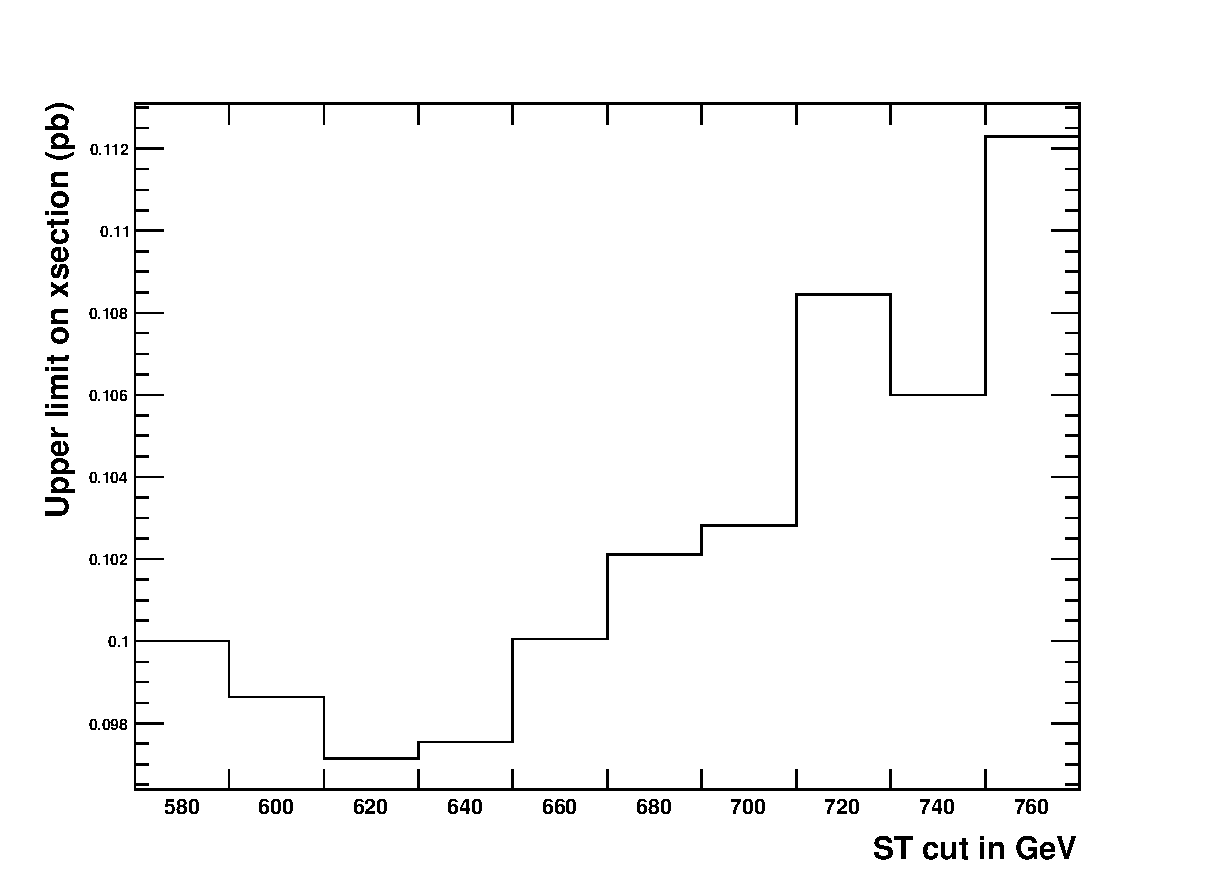
\includegraphics{plots/xSecLimit_M400.eps}} \\
    \caption{\small \sl Upper limit on the signal cross section for a range of $S_T$ cuts for LQ mass of 400 GeV. 
      The optimal cut (620 GeV) is found to be independent from the addition of systematic uncertainties in the 
      number of signal and background events.}
    \label{fig:optimization}
  \end{center}
\end{figure}
%

%\end{document}
